%!TeX encoding = UTF-8 Unicode
%!TeX spellcheck = en-UK
% !TeX root = Perrinet26mnesis.tex
% -*- coding: UTF-8; -*-
%%%-----------------------------------------------------------------
\begin{figure}[!t]
\centering
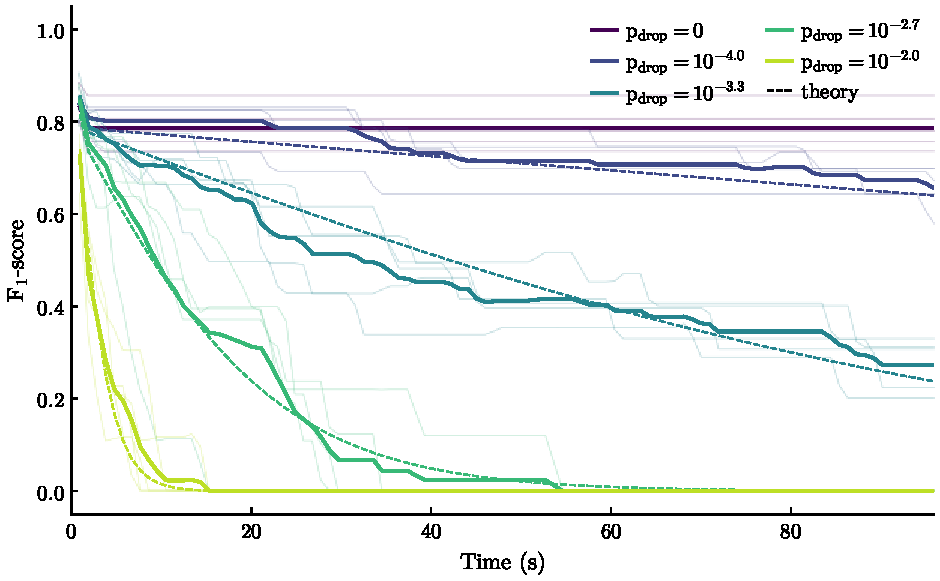
\includegraphics[width=\linewidth]{periodic_scores.pdf}
\caption{Free replay of periodic motifs under transmission failures. The motifs are made periodic by copying their trigger window (the first $D=41$ steps) onto their last $D$ steps, so that the chain of Spiking Motifs closes on itself with a period of $T-D=959$ steps of $1\,\mathrm{ms}$, that is $0.959\,\mathrm{s}$, about one second. After a single noisy trigger window ($p_\mathrm{flip} = 0.01$), each spike emitted by the network is removed from the recurrent input with probability $p_\mathrm{drop}$, and the network runs freely for $100$ periods ($95.9\,\mathrm{s}$). Each curve is one level of $p_\mathrm{drop}$, as given by the legend: $p_\mathrm{drop} = 0$ and four log-spaced levels from $10^{-4}$ to $10^{-2}$. Thin lines show the $5$ seeded realisations of each level, thick lines their mean. Each period is scored ($F_1$ score computed on the spikes of the $M=16$ motifs pooled together) against the frozen motif, and plotted at the time at which the period ends, counted from the end of the trigger window. Dashed lines: prediction of the cascade model (Section~\ref{sec:robustness}), in which each spike of a sustained replay is a new ignition test, so that the replay survives $t$ steps with probability $\exp(-ht)$. Without failures, the score settles on the limit cycle after the first period; with failures, the replay decays with a mean lifetime $1/(hP)$ of about $280$, $60$, $12$ and $2$ periods at the four non-zero levels.}\label{fig:periodic}
\end{figure}
%%%-----------------------------------------------------------------
